\section{Multiple Tubes Constant Mass Flowrate}
Next the system is formulated for multiple tubes. This is done by finding the individual velocity/mass flowrate that will be flowing through each pipe. The team assumes that the waste water and internal flowrate coming into the heat exchanger will be split evenly to each 10 meter long heat exchanger. All other constants besides number of pipes will be held constant. As seen in part 1 the Nusslet number for each will be calculated using the Reynolds number. This Reynolds number uses a mass flowrate that is a ``fraction'' of the total that comes into the system.
% Reynold numbers for pipes
\begin{subequations}
\begin{eqnarray}
 { Re }_{ D } =\frac { \rho { D }_{ i }{ V }_{ i,partial } }{ \mu  } =\frac { { D }_{ i }{ \dot { m }  }_{ i } }{ N\mu { A }_{ c } } \\ 
 { Re }_{ Dh } =\frac { \rho { D }_{ h }{ V }_{ i,partial } }{ \mu  } =\frac { { D }_{ h }{ \dot { m }  }_{ o } }{ N\mu { A }_{ c } } 
\end{eqnarray}
\end{subequations}
%
Using the above equations and equations \eqref{eq_part_1_5} and \eqref{eq_part_1_6} the Nusslet number can be calculated and thus the convection coefficients can be finally calculated. When the total resistance is calculated the number of tubes becomes important again. The convection coefficient calculated is for a single pipe, thus we want to apply this to the entire surface area of the system. This calculation of the total resistance can be seen below.
%
\begin{equation}
    { R }_{ total }=\frac { 1 }{ { \bar { h }  }_{ i }N{ A }_{ s } } +\frac { 1 }{ { \bar { h }  }_{ o }N{ A }_{ s } } 
\end{equation}
%
\begin{figure}[H]
    \centering
    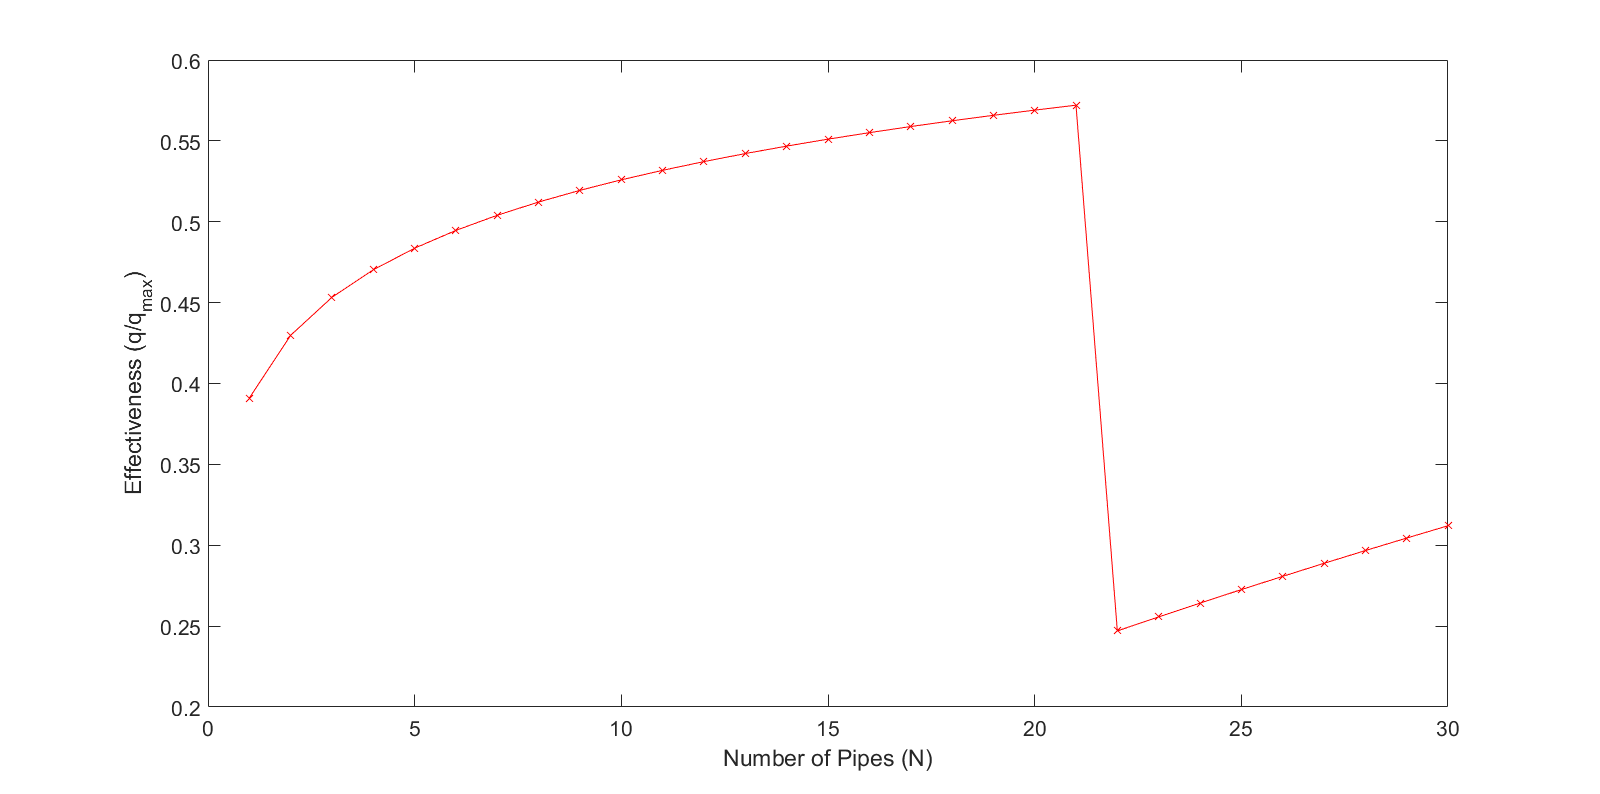
\includegraphics[height=3.5in]{pictures/part_2_2m2_effectiveness.png}
\end{figure}
%
\noindent
From the results, it is observed that the effectiveness of the system drops significantly when using approximately 22 tubes. This is because the outside Reynolds number, see figure below, transitions from turbulent to laminar which causes the Nusslet number to change in the process. Note that this effectiveness was calculated with a constant cold water mass flowrate of 2 kg/s.
%
\begin{figure}[H]
    \centering
    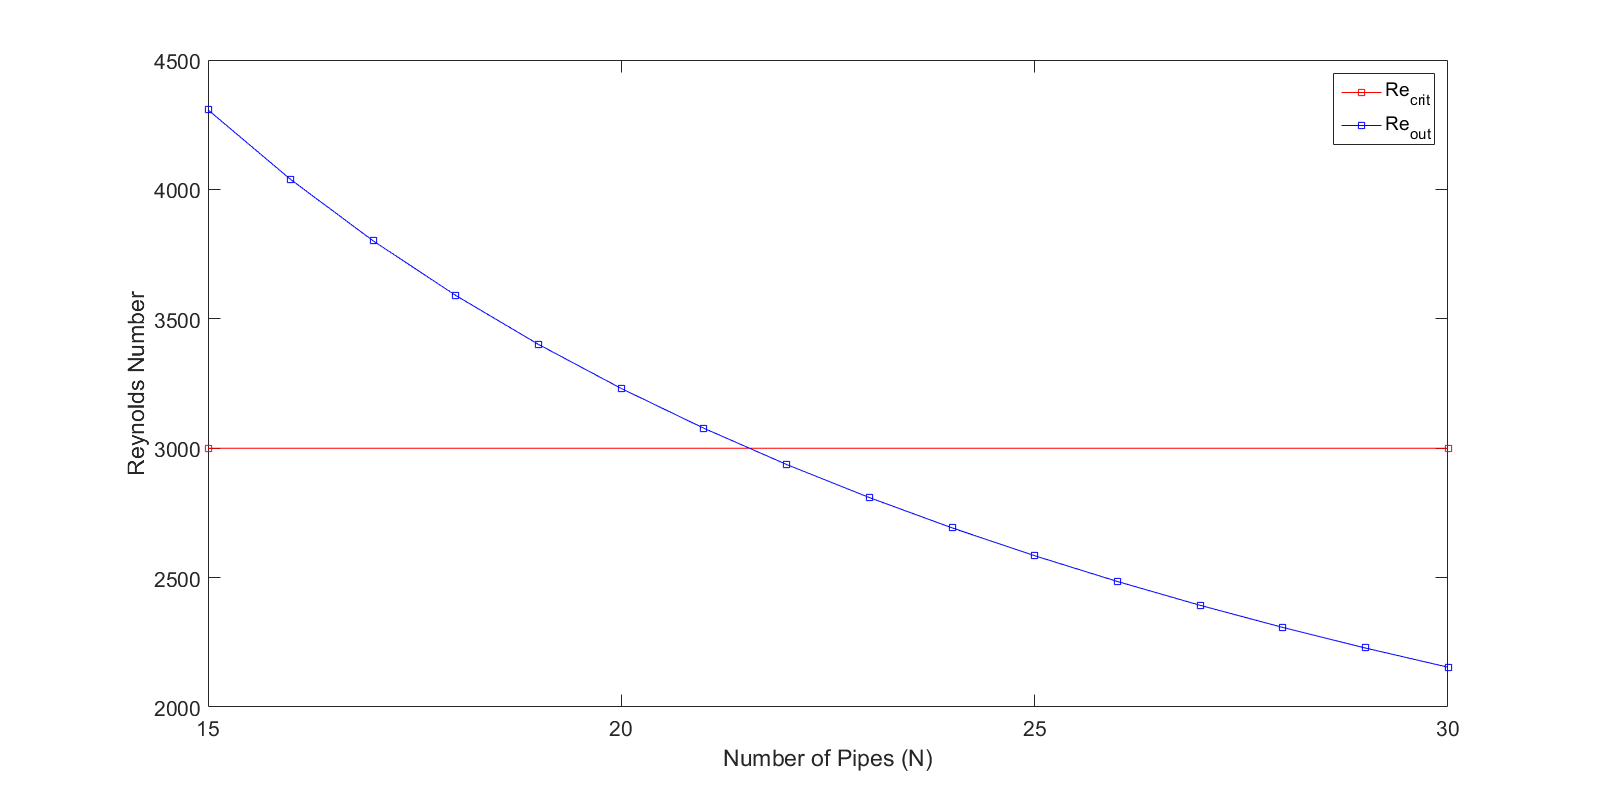
\includegraphics[height=3.5in]{pictures/part_2_2m2_reynolds_crit.png}
\end{figure}
%
\noindent
This is an interesting numerical problem with the equations that are used to simulate the flow. Because we do not have an equation representing the transition state from turbulent to laminar we instead have this piecewise function that causes jumps like theses. We can gain insight to how the system would preform with these number of tubes by looking at how the outlet temperatures change with the number of tubes.
%
\begin{figure}[H]
    \centering
    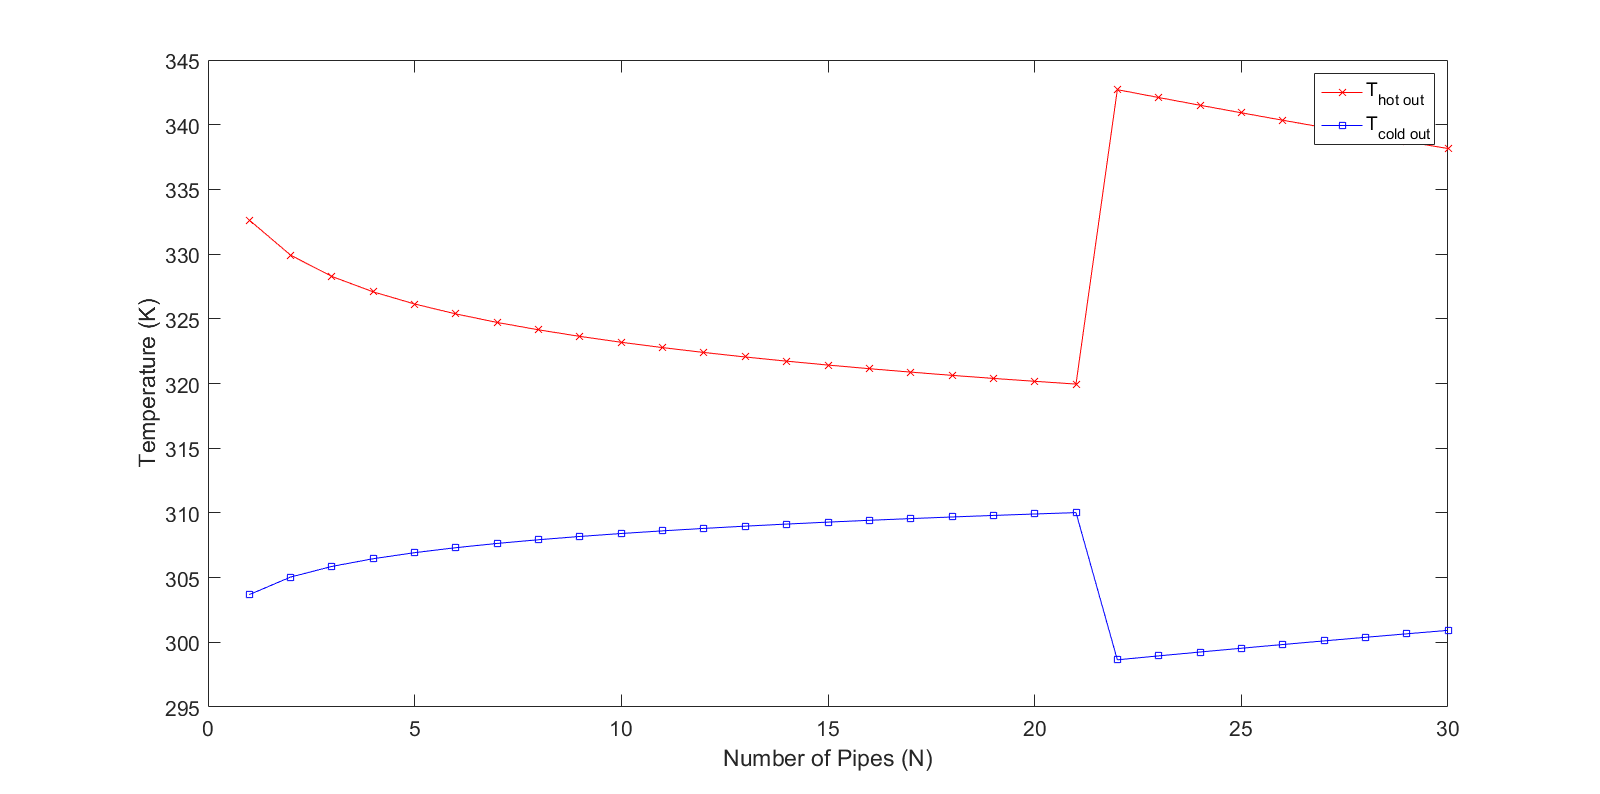
\includegraphics[height=3.5in]{pictures/part_2_2m2_temps.png}
\end{figure}
%
\noindent
As seen above the outlet temperatures provide an interesting insight into the behavior of the system. We can see that there is the expected jump at 22 tubes, but it is interesting to see that the outlet temperatures actually ``reset'' to close to their inlet temperatures. This is tied to the Reynolds number, and that the outside flow has now transitioned from turbulent to laminar, and thus it has a decrease in its ability to transfer heat.